\section{Garbage Collection}
\label{sec:garbage_collection}

As seen in Specification~\ref{alg:sor_set}, update procedures add tuples to
either $A$ or $R$ sets, which lead to an increase of database in size. If we
want to always have a complete history for a replica, then the behavior may
conform to these requirements. However, due to space constraints, this
assumption is usually not practical. Hence, this section introduces an automatic
garbage collection mechanism for removing, or \textit{expiring}, tuples from
these sets after a specified time interval. To this extent, elements are
considered to have limited lifetime in the store, setting that can be decided on
a case-by-case basis. For example, if the set tracks statistics about IP
addresses used for logging into a user account, we may not be interested in IPs
older than one month.

Any $(e, t, rc, rs) \in A$ in the SOR-Set will be referred to as an
\textit{ADD(e)} tuple and any $(e, t, rc, rs, t', rc', rs') \in R$ as an
\textit{RMV(e)} tuple. These tuples are generated either when the client calls
\textit{add} and \textit{remove} methods, or through the synchronization
process. Lookup semantics states that $\textit{lookup}(e)$ should return
\textit{true} if $e$ is in the SOR-Set and \textit{false} otherwise. The
following theorem on tuples expiration can now be formulated.

\begin{theorem*}[\textbf{Tuples expiration}]
\begin{itshape}
If, at any given shard, the tuples corresponding to any element $e$,
\textit{ADD(e)} and \textit{RMV(e)}, are expired in the same order in which they
were originally inserted, then the lookup semantics are preserved.
\end{itshape}
\end{theorem*}

\begin{proof}
Let us first consider update operations occurring at one replica with no
synchronization taking place. There are two cases: i) $ADD(e) \rightarrow
RMV(e)$, meaning \textit{ADD(e)} is inserted before \textit{RMV(e)}. The
expected return value for $\textit{lookup}(e)$ after these operations are
executed is evidently \textit{false}. If \textit{ADD(e)} expires first and
\textit{RMV(e)} expires later, then the semantics does not change. If, however,
expiration occurs in reverse order, there will be a time window when
\textit{ADD(e)} is present, but \textit{RMV(e)} not. In this interval, a
$\textit{lookup}(e)$ call will return \textit{true}, which will change the
expected semantics. ii) $RMV(e) \rightarrow ADD(e)$. The proof follows the same
rationale.

Consider now the situation when tuples propagate from one shard to another.
Again there are two cases: i) $ADD(e) \leadsto RMV(e)$, which symbolizes that
\textit{ADD(e)} was originally inserted at one shard, fetched through replica
synchronization and then a \textit{RMV(e)} was inserted locally. As soon as the
remote \textit{ADD(e)} is inserted in the local set, this case reduces to the
corresponding sequential one from before: $ADD(e) \rightarrow RMV(e)$ and both
tuples should be expired in the same order in which were originally inserted.
If the \textit{RMV(e)} is inserted before \textit{ADD(e)} reaches the local
shard, these updates are concurrent and $ADD(e)$ wins: $\textit{lookup}(e)$ will
return \textit{true} as long as the $ADD(e)$ is not expired, which is what we
expect. ii) $RMV(e) \leadsto ADD(e)$. Similarly, the case reduces to the
sequential $RMV(e) \rightarrow ADD(e)$.
\end{proof}

\begin{figure}[b!]
  \centering
  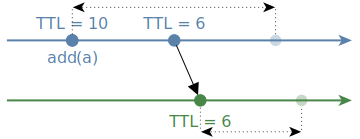
\includegraphics[width=0.6\linewidth]{garbage-collection}
  \caption{Preserving TTL on updates propagation}
  \label{fig:garbage-collection}
\end{figure}

The following changes could be made to the SOR-Set specification in order to
include an automatic, asynchronous garbage collection while maintaining the
lookup semantics. We associate a \textit{time-to-live} (TTL) value with each
tuple when it is inserted into the corresponding set through an \textit{add} or
\textit{remove}. This value represents the time interval from the moment it was
inserted after which the tuple will expire. In this way, tuples older than a
specified period are considered to be no longer relevant and can be safely
discarded. Data stores such as Redis~\cite{redis} or Cassandra~\cite{cassandra}
offer support for setting TTL attributes to records and automatic removal for
expired ones. Otherwise, a simple periodic scan-and-remove process on the
database can be used. To ensure that tuples corresponding to $e$ expire in the
order in which they were added, first, it is sufficient to stamp them with the
same value $TTL(e)$. Tuples corresponding to different values may be stamped
with different TTLs. Second, as shown in Fig.~\ref{fig:garbage-collection}, when
copying the tuples to other shards, their remaining TTL should be preserved,
i.e. the current TTL at the remote replica is transferred together with the
tuple to the local replica. By doing this, tuples will expire at the local
replica in the same order as they do at the remote one.

We note that it is not a requirement for having the same physical clock speed on
all machines or for having their clocks periodically synchronized. What is
needed is only a partial order on the tuples expiration as stated by the above
theorem. Preserving the TTLs for tuples when propagating them across different
shards evidently does not imply that there is a global time point when all
copies of one tuple are expired simultaneously. In fact, copies of the tuples in
local cluster will expire shortly after the original ones in remote cluster have
expired. However, this does not invalidate the lookup semantics according to the
tuples expiration theorem.

\begin{IEEEproof}[Garbage collection maintains the CRDT properties]
We consider first the case when no sharding is used. A new partial order can be
defined by the relation $S_{1} \sqsubseteq S_{2} \iff S_{1} \subseteq S_{2} \lor
S_{1} \equiv (S_{1} \cap S_{2})$. The first term holds when no tuples are
expired and thus either \textit{add} or \textit{remove} operation increases the
corresponding set like before. If by the time we apply any operation, some
tuples are expired from $S_{1}$, then the states containing old non-expired
tuples from before and after the update are considered equivalent, i.e. any
$\textit{lookup}(e)$ method on either $S_{1}$ or $S_{1} \cap S_{2}$ returns the
same result. It is easy to see that, relative to $\sqsubseteq$, the updates
always advance the states in the partial order. Taking sharding into account, we
can simply consider the union of all $A$ and, respectively, $R$ sets in one
cluster as in Specification~\ref{alg:sor_set}: $S_{i} = \bigcup_{\forall j \in
\{1,\ldots,|rc_{i}|\}} S_{i}^{j}$, where $S$ is $A$ or $R$. From this point, the
proof follows the same rationale as for the SOR-Set.
\end{IEEEproof}